\section{Reconnaissance de visage}
\begin{frame}
  \frametitle{Detection de visage}
  \begin{columns}[c]
    \begin{column}[T]{.5\textwidth}
      \begin{itemize}
        \item Utilisation d'OpenCV
          \begin{itemize}
            \item open source computer vision library
          \end{itemize}
        \item Utilisation de classifieur pour la detection de visage
          \begin{itemize}
            \item Obtetion d'un cercle (rayon et centre)
          \end{itemize}
      \end{itemize}
    \end{column}
    \begin{column}[T]{.5\textwidth}
      \begin{figure}
        \begin{center}
          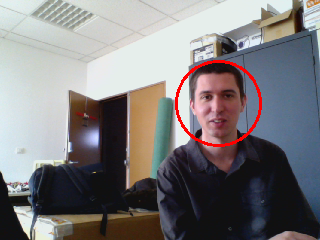
\includegraphics[width=5cm]{image/faceDetection.png}
          \caption{Example de detection de visage}
        \end{center}
      \end{figure}
    \end{column}
  \end{columns}   
\end{frame}

\begin{frame}
  \frametitle{}
\end{frame}
